\documentclass[reprint, english, nofootinbib]{revtex4-2}

\usepackage{graphicx}
\usepackage{subfig}
\usepackage[colorlinks=true,urlcolor=blue,citecolor=blue]{hyperref}
\usepackage{physics}
\usepackage{amsmath}
\usepackage{amssymb}
\usepackage{amsbsy}
%\usepackage{bbold}
\usepackage{subfig}

\usepackage{blindtext}
\usepackage{tikzducks}
\usepackage{tikz}
\usepackage{pgfplots}
\usepackage{listings}

\graphicspath{{../figs/}}

\begin{document}
\title{Classification and Regression\\
\normalsize{From Linear and Logistic Regression to Neural Networks}}

\author{Nicholas Karlsen}
\affiliation{University of Oslo}
\author{Thore Espedal Moe}
\affiliation{University of Oslo}
\date{\today}

\begin{abstract}
%%%% ABSTRACT
In this paper we implement from scratch a fully connected Feed-Forward Neural Network (FFNN) and investigate its application to function approximation and classification. To wit, we study the prediction/reconstruction of a set of terrain data from a subset of data-points as an example of function approximation, and we study the classification of hand-written digits 0-9 from the MNIST-dataset. As it is in a sense the motor of our neural network, we also look in some detail at the properties of the Stochastic Gradient Descent (SGD) method and its variant siblings. The performance of our network on the reconstruction of terrain data is compared and contrasted with previous results obtained via linear-regression methods. For the classification case the comparison is made with results from a logistic-regression based classifier that we also implement from scratch. We find that our FFNN fairly easily gives excellent results for the classification problem, and that it is significantly more accurate than our logistic-regression classifier; at least without further fine-tuning of the logistic classifier . For the terrain-predictions we observe, for some setups, sizable improvements over the previous results from linear-regression, but only after rather extensive fine-tuning of the network's hyper-parameters
%%%%%%%

\end{abstract}

\maketitle

\section{Introduction}


Neural networks are among the most hyped techniques in modern machine learning. Being that they are extremely flexible and applicable to a wide range of problems from general function approximations to all sorts of classification tasks, this is hardly surprising. The blessing of flexibility can, however, be a curse in disguise as it gives rise to veritably vast range of hyper-parameters that must be tuned to the specific problems at hand. They have great potential, but the art of applying them optimally can at times appear akin to black magic.

In the present work we implement from scratch a Feed-Forward Neural Network (FFNN), aiming to explore its application both to linear-regression type problems and to classification tasks. We hope to gain some sense for the relative importance and the general effects of the various hyper-parameters the network can take in.

In somewhat simple terms, one can consider neural networks to be a collection of various weighting parameters that combine the inputs to the network in complicated non-linear ways to produce a predictive output. In order for the network to make useful predictions, it must be trained. That is, its weights must be optimized in some problem-specific way. In our present case, this optimization/training is driven by Stochastic Gradient Descent (SGD) methods. In a certain sense the neural network can be thought of as a car frame, translating the work of the SGD engine into movement/improved predictions. As such we will begin with testing the tuning of SGD (and some of its myriad siblings) applied to a simple linear-regression type problem where we have analytical solutions for the optimal model parameters. The goal is to gain insights into the properties of the SGD-type engines, which hopefully can guide our investigations of the full networks.

Armed with insights from the investigation of the SGD-methods, we turn to study the application of our neural network to a linear-regression type problem, namely the terrain-prediction considered in \cite{4155_project_1}. We vary a select set, guided by the results for the SGD-methods, of the network's hyper-parameters and try to find combinations which give better predictions than those obtained in \cite{4155_project_1}. The flexibility of neural networks can be expected to better predict such highly non-linear functions than regular (polynomial) linear-regression; but finding the combinations of hyper-parameters which actually perform better than plain old linear-regression is not trivial.

Subsequently we test the application of our network on a classification problem, specifically the classification of hand-written digits 0-9 from the MNIST data set. Once again we tune our network in an effort to obtain the best possible performance we can manage. In order to compare the neural network's results with another machine learning method, we then implement a simple multinomial logistic regression and apply it to the same classification problem.

Finally we summarize and compare how the different methods perform, both in terms of accuracy and computational speed, but also in terms of the time cost and difficulty for the user to find reasonable hyper-parameters. We do not aim to make definite statements as to which method is "best" since that very much varies from case-to-case; both in terms of how the various aspects like accuracy and computational speed are valued, but also in terms of how the various hyper-parameters relate to the problem at hand. Instead we wish point out some tendencies of a hopefully somewhat general nature, which can serve as a guidelines for which methods one might prefer to try first for a given case.


\section{Theory}
\subsection{Gradient Descent}
\noindent
Consider a cost function in the form
\begin{equation}
    C(\pmb Y, \tilde{\pmb Y}(\pmb w)) = \frac{1}{N}\sum_{i=1}^{N}c_i(\pmb y_i, \tilde{\pmb y}(\pmb w)_i)
\end{equation}
which quantifies the error for some data set $\pmb Y = \left\{\pmb y_1, \dots, \pmb y_N\right\}$ with respect to a corresponding set of modeled data $\tilde{\pmb Y}(\pmb w) = \left\{\tilde{\pmb y_1}(\pmb w), \dots, \tilde{\pmb y}_N(\pmb w)\right\}$, where $\pmb w$ denotes the free parameters of the model.

Since we can not in general expect to have a way of minimizing the cost analytically, we may in stead optimize it by gradient descent (GD), where the set of free parameters $\pmb w$ are initialized in some way, and then incremented by
\begin{equation}\label{eqn: GD}
    \pmb w^{(k+1)} = \pmb w^{(k)} - \eta \nabla_{w}C\qty(\pmb Y, \tilde{\pmb Y}(\pmb w))
\end{equation}
for either a set number of epochs or in practice, until $\norm{\pmb w^{(k+1)} - \pmb w^{(k)}}_2< \varepsilon$, some tolerance. We also have the parameter $\eta \in \mathbb R_{>0}$, often called the learning rate, which can either be constant, or change wrt. $k$.

A notable, and very substantial drawback of GD is that it will always converge to a local minima for a given data set \& initial weights, which for a particularly complicated high dimensional parameter space can not be expected to correspond to the global minima in general. This issue, along with many others \cite[pp.15-16]{Mehta_2019} motivates modifications to the GD method.

\subsubsection{Stochastic Gradient Descent}
\noindent
One attempt at remedying the problems of GD is the so-called \textit{Stochastic Gradient Descent} (SGD), in which stochasticity is introduced to the gradient descent by instead of performing GD on the entirety of $\pmb Y$, it is performed on individual, randomly sampled points $\pmb y_i$ with replacement, and updating the weights for each individual sample.
It turns out that doing SGD in this way generally leads to faster, and better convergence compared to the regular GD, with the added benefit of being computationally faster. It is worth noting however that it is often observed that doing SGD without replacement can yield faster convergence, and is in practice often done this way. The exact reasoning behind this remaining an open question \cite{shamir2016withoutreplacement}\cite{pmlr-v97-nagaraj19a}. For simplicity, we have opted to conform to this norm and will be performing SGD without replacement.

\subsubsection{SGD with Mini-Batches\label{sect: SGD with mini-batches}}
\noindent
Yet another modification of the SGD consists of performing the SGD on random subsets $\pmb Y_{MB} \subset \pmb Y$, rather than individual points $\pmb y_i$. These subsets are often called \textit{Mini-Batches} (MB), and their introduction may again improve the performance of SGD. To elaborate, this is performed by randomly splitting $\pmb Y$ into a set of mini-batches where each subset has $\approx N_{B}$ elements\footnote{If $\pmb Y$ is not exactly divisible, one may simply distribute the extra $\pmb y_i$ equally among the batches}. GD is then performed on each of the subsets, updating the weights each time. Once the subset has been exhausted, $\pmb Y$ is again randomly sampled to construct another similar set of mini-batches, where each shuffling of the mini-batches constitutes an epoch of the algorithm.

The choice of $N_{B}$ somewhat decided by trial and error and is also strongly linked to the choice of learning rate $\nu$. However, it is usually chosen as relatively small number relative to the full dataset as to yield the benefits of the SGD method. One may also, as discussed in this excellent lecture by \textcite{ManyBodyML} intuitively link SGD to statistical mechanics, with the ratio $\eta / N_{B} \propto T$; representing an "effective temperature". Thus having small mini-batch sizes corresponds to a high effective temperature; where the system will be able to explore a much larger portion of the parameter space. Then by either increasing $N_B$, or decreasing $\eta$ one may slowly lower the effective temperature; annealing the system into the global minima. For the full justification of this view; we refer the reader to \textcite{ManyBodyML}.

Common choices for $N_B$ is often in the order of $\sim 10-100$, with larger batches often yields diminishing returns in terms of the performance gain along with a larger computational cost. Further, choosing batch sizes as powers of 2 may yield slight performance gain by virtue of how computer hardware works \cite{Aggarwall}.

\subsubsection{Learning Rate Adjustment}
\noindent
As somewhat motivated by the intuition motivated in the previous section, it is often quite useful to be able to adjust the learning rate of SGD over the epochs, as this will in principle allow the algorithm to initially very rapidly explore the parameter space, prior to relaxing slowly into the (hopefully) global minima as the learning rate is decreased.

One such scheme is the inverse decay, where the learning rate evolves like
\begin{equation}
    \eta\qty(t) = \frac{\eta_0}{1 + \gamma t}
\end{equation}
where $\eta_0$ is the initial learning rate, $t$ the current epoch and the decay rate $\gamma$ which controls the rate at which the learning rate will decrease. Similarly; we may also evolve the learning rate by as exponential decay as
\begin{equation}
    \eta(t) = \eta_0 e^{-\gamma t}
\end{equation}
where the appropriate choice must be determined on a per-dataset basis as the convergence of SGD will vary wildly. An additional, much more involved technique is to run the SGD for a certain number of epochs, then manually readjusting the learning rate, either as a constant or by the above methods, then running for another set of epochs. Whilst this sort of technique where one manually hand-tunes the hyper-parameters requires much attention from the user, it may yield good results and even enable some of the simpler schemes to outperform some of the more sophisticated, adaptive schemes \cite{zhang2018yellowfin}.

\subsubsection{SGD Variants}
\noindent
Beyond the basic iteration defined by Eqn.~\ref{eqn: GD}, there exists a large number of alterations beyond just scaling the learning rate which in some way aim to improve the convergence of SGD. Some of which generally yield performance gains, whilst other may yield performance gains for particular types of problems. Perhaps the simplest of which is SGD with momentum (SGDM), which as the name suggests adds some parameter to the update rule which somehow attempts to respect the current rate at which the algorithm is traversing parameter space; speeding past shallow dips and slowing down for deep, narrow ones. Much akin to the physical quantity from which it is named. The update scheme may then be summarized by the following equations
\begin{align}\label{eqn: SGDM}
    \begin{split}
        \Delta \pmb w^{(k)} &= p \Delta\pmb w^{(k-1)} - \eta \nabla_wC(\pmb Y, \tilde{\pmb Y}(\pmb w)) \\
        \pmb w^{(k+1)} &= \pmb w^{(k)} + \Delta\pmb w^{(k)}
    \end{split}
\end{align}
where the momentum $p$ is usually set in the interval $[0, 1]$. Whilst simple, this scheme often yields significant performance gains over the standard constant learning rate methods, which in practice is rarely used \cite{Mehta_2019}. There also exists a plethora of other sophisticated schemes that in some way aims to increase the convergence rate of SGD, like the adaptive gradient (AdaGRAD), in which the learning rate is down-scaled by a cumulative history of the magnitude gradient. There is also the Root mean squared propagation (RMSProp) which works in a similar way to AdaGRAD by adapting the learning-rate to the gradient, but has an additional hyper-parameter which lets it "forget" older gradients. Common to many of these schemes however; is that they are often domain specific, and while they may yield exceptional performance for certain problems, there is no universal best choice.

\begin{figure}[h!tb]
    \center
    \vspace{5mm} % To avoid touching the preceding text
    


\tikzset{every picture/.style={line width=0.75pt}} %set default line width to 0.75pt

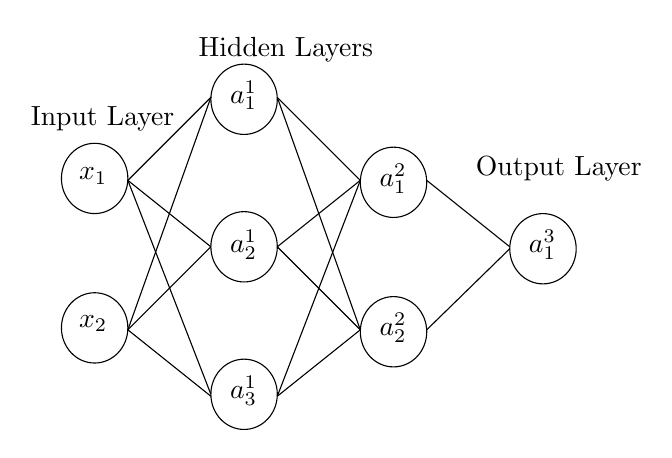
\begin{tikzpicture}[x=0.6pt,y=0.6pt,yscale=-1,xscale=1]
%uncomment if require: \path (0,484); %set diagram left start at 0, and has height of 484

%Flowchart: Connector [id:dp6019250960891445]
\draw  [fill={rgb, 255:red, 255; green, 255; blue, 255 }  ,fill opacity=1 ] (40,112.83) .. controls (40,101.14) and (48.95,91.67) .. (60,91.67) .. controls (71.05,91.67) and (80,101.14) .. (80,112.83) .. controls (80,124.52) and (71.05,134) .. (60,134) .. controls (48.95,134) and (40,124.52) .. (40,112.83) -- cycle ;
%Flowchart: Connector [id:dp8334547170271857]
\draw  [fill={rgb, 255:red, 255; green, 255; blue, 255 }  ,fill opacity=1 ] (40,202.83) .. controls (40,191.14) and (48.95,181.67) .. (60,181.67) .. controls (71.05,181.67) and (80,191.14) .. (80,202.83) .. controls (80,214.52) and (71.05,224) .. (60,224) .. controls (48.95,224) and (40,214.52) .. (40,202.83) -- cycle ;
%Flowchart: Connector [id:dp7153685420206096]
\draw  [fill={rgb, 255:red, 255; green, 255; blue, 255 }  ,fill opacity=1 ] (130,65.17) .. controls (130,53.48) and (138.95,44) .. (150,44) .. controls (161.05,44) and (170,53.48) .. (170,65.17) .. controls (170,76.86) and (161.05,86.33) .. (150,86.33) .. controls (138.95,86.33) and (130,76.86) .. (130,65.17) -- cycle ;
%Flowchart: Connector [id:dp5622283646258179]
\draw  [fill={rgb, 255:red, 255; green, 255; blue, 255 }  ,fill opacity=1 ] (130,154) .. controls (130,142.31) and (138.95,132.83) .. (150,132.83) .. controls (161.05,132.83) and (170,142.31) .. (170,154) .. controls (170,165.69) and (161.05,175.17) .. (150,175.17) .. controls (138.95,175.17) and (130,165.69) .. (130,154) -- cycle ;
%Flowchart: Connector [id:dp16862921724788715]
\draw  [fill={rgb, 255:red, 255; green, 255; blue, 255 }  ,fill opacity=1 ] (130,242.83) .. controls (130,231.14) and (138.95,221.67) .. (150,221.67) .. controls (161.05,221.67) and (170,231.14) .. (170,242.83) .. controls (170,254.52) and (161.05,264) .. (150,264) .. controls (138.95,264) and (130,254.52) .. (130,242.83) -- cycle ;
%Flowchart: Connector [id:dp4149695521858179]
\draw  [fill={rgb, 255:red, 255; green, 255; blue, 255 }  ,fill opacity=1 ] (220,115.17) .. controls (220,103.48) and (228.95,94) .. (240,94) .. controls (251.05,94) and (260,103.48) .. (260,115.17) .. controls (260,126.86) and (251.05,136.33) .. (240,136.33) .. controls (228.95,136.33) and (220,126.86) .. (220,115.17) -- cycle ;
%Flowchart: Connector [id:dp840876892841651]
\draw  [fill={rgb, 255:red, 255; green, 255; blue, 255 }  ,fill opacity=1 ] (220,205.17) .. controls (220,193.48) and (228.95,184) .. (240,184) .. controls (251.05,184) and (260,193.48) .. (260,205.17) .. controls (260,216.86) and (251.05,226.33) .. (240,226.33) .. controls (228.95,226.33) and (220,216.86) .. (220,205.17) -- cycle ;
%Flowchart: Connector [id:dp10784935111712701]
\draw  [fill={rgb, 255:red, 255; green, 255; blue, 255 }  ,fill opacity=1 ] (310,155.17) .. controls (310,143.48) and (318.95,134) .. (330,134) .. controls (341.05,134) and (350,143.48) .. (350,155.17) .. controls (350,166.86) and (341.05,176.33) .. (330,176.33) .. controls (318.95,176.33) and (310,166.86) .. (310,155.17) -- cycle ;
%Straight Lines [id:da7667435970573455]
\draw    (80,114) -- (130,154) ;
%Straight Lines [id:da48448129133283535]
\draw    (170,154) -- (220,114) ;
%Straight Lines [id:da4471635916327932]
\draw    (260,114) -- (310,154) ;
%Straight Lines [id:da5105417767244789]
\draw    (80,204) -- (130,244) ;
%Straight Lines [id:da6281305874976782]
\draw    (170,154) -- (220,204) ;
%Straight Lines [id:da9404110386397875]
\draw    (260,204) -- (310,155.17) ;
%Straight Lines [id:da669909761533326]
\draw    (130,154) -- (80,204) ;
%Straight Lines [id:da03861624272354913]
\draw    (80,204) -- (130,64) ;
%Straight Lines [id:da7865539839743194]
\draw    (80,114) -- (130,64) ;
%Straight Lines [id:da006395151871996019]
\draw    (170,64) -- (220,114) ;
%Straight Lines [id:da6703248416054105]
\draw    (170,64) -- (220,204) ;
%Straight Lines [id:da568582824840071]
\draw    (170,244) -- (220,204) ;
%Straight Lines [id:da5603512527475397]
\draw    (170,244) -- (220,114) ;
%Straight Lines [id:da15589575659778376]
\draw    (80,114) -- (130,242.83) ;

% Text Node
\draw (49,105) node [anchor=north west][inner sep=0.75pt]    {$x_{1}$};
% Text Node
\draw (49,194) node [anchor=north west][inner sep=0.75pt]    {$x_{2}$};
% Text Node
\draw (140,52.33) node [anchor=north west][inner sep=0.75pt]    {$a^{1}_{1}$};
% Text Node
\draw (140,142.33) node [anchor=north west][inner sep=0.75pt]    {$a^{1}_{2}$};
% Text Node
\draw (140,230) node [anchor=north west][inner sep=0.75pt]    {$a^{1}_{3}$};
% Text Node
\draw (230,102.33) node [anchor=north west][inner sep=0.75pt]    {$a^{2}_{1}$};
% Text Node
\draw (230,192.33) node [anchor=north west][inner sep=0.75pt]    {$a^{2}_{2}$};
% Text Node
\draw (320,142.33) node [anchor=north west][inner sep=0.75pt]    {$a^{3}_{1}$};
% Text Node
\draw (20,68) node [anchor=north west][inner sep=0.75pt]   [align=left] {Input Layer};
% Text Node
\draw (288,98) node [anchor=north west][inner sep=0.75pt]   [align=left] {Output Layer};
% Text Node
\draw (185,35) node   [align=left] {\begin{minipage}[lt]{74.80000000000001pt}\setlength\topsep{0pt}
Hidden Layers
\end{minipage}};


\end{tikzpicture}

    \caption{\label{fig: NN Fig} Visual representation of a simple neural network with $2$ inputs, $2$ hidden layers with $3$, $2$ neurons respectively and an output layer with a single neuron.}
\end{figure}

\subsection{Neural Networks}
\noindent
Neural Networks are a class of algorithms in which a set of nodes, often referred to as Neurons, are connected as a weighted graph. Which as the name may suggests, aims to emulate behaviour similar to that of the human brain. Each of the nodes in this graph is then activated by an activation function, which takes the weighted input of all of its connected graphs like
\begin{equation}
    a = \sigma\qty(w_1 a_1' + w_2 a_2' + \dots + w_n a_n' + b)
\end{equation}
where $w_i$, $a_i'$ denotes the weights and activations of the connected nodes, and $\sigma$ the activation function of the node, which is chosen differently depending on the problem at hand. Lastly, we have also have a bias, $b$, which simply shifts the activation of the Node in the case of a binary activation, or tn the case where the activation function is chosen to be the identity function, the bias is simply the intercept.

The simplest type of neural network is the \textit{Feed-Forward Neural Network} (FFNN), which is a directed graph, consisting of layers where every neuron in the preceding layer is connected to every neuron in the following layer as depicted in Fig.~\ref{fig: NN Fig}, which is directed going from left to right.

As the name may suggest, the input layer is where the input data starts out, before being fed forward through the hidden layers of the network, weighted in-between each node before reaching the output layer, the final model. In a similar fashion to other methods of supervised learning, the neural network must first undergo a process of training to obtain a suitable set of weights and biases. This is done by optimizing the all of the weights and biases in the network wrt to a chosen cost function usually by SGD. However, due to the costly nature of evaluating all of these cost functions; an algorithm which cleverly exploits the chain rule of differentiation has been developed to very efficiently compute all of the gradients in the network in a process which is called backpropagation.Neural Networks and Deep Learning

\subsubsection{Backpropagation}
\noindent
We base our explanation of the backpropagation algorithm following more or less directly from \textcite{Nielsen} and \textcite{Mehta_2019}, referring the reader to those texts for the finer details and derivations of how the algorithm actually works, focusing instead on the computational aspects in the present texts. However, in short; the algorithm may be summarized as a clever use of the chain rule of differentiation.

Before we start, we first define a few quantities central to the network. First, we have the set of weights connecting each node in the network
\begin{equation}
    \{w^{1}_{jk}, \dots, w_{jk}^L\}
\end{equation}
where in a somewhat sloppy notation the $j, k$ indices denote the number of neurons in the current and previous layers respectively, thus spanning a different range for each $l$. We also define the set of inputs
\begin{equation}
    \{z_j^1, \dots, z_j^L\}
\end{equation}
which again adheres to the same convention of $j$ denoting the number of neurons in the current layer. These inputs then gets fed into the activation function $\sigma(z_j^l)$ of their corresponding neurons yielding the set of activations
\begin{equation}
    \{a_j^1, \dots, a_j^L\}
\end{equation}
where notably the activation function used in the output layer may differ from the one used in the hidden layers. We denote this special, output activation function as $\tilde \sigma(z_j^L)$.

We then start the backpropagation algorithm by first computing the response of each of the neurons in the network by the Feeding the input data forward in the network, starting with the first hidden layer, which is activated directly by the input data $X_p$ like
\begin{align}\label{eqn: FeedForward Initial}
    \begin{split}
        z^1_j &= w^1_{jk}X_k + b^1_j \\
        a^1_j &= \sigma(z^1_j)
    \end{split}
\end{align}
where we adopt the Einstein summation convention by summing over repeated indices.
We then similarly compute
\begin{align}
    \begin{split}
        z^l_{j} &= w^l_{jk}a^{l-1}_k + b^l_j \\
        a^l_{j} &= \sigma(z^l_{j})
    \end{split}
\end{align}
for hidden layers $l = 2, \dots, L$. Then, for the output layer we compute
\begin{align}
    \begin{split}
        z^{L}_j &= w^{L}_{jk}a^{L-1}_k + b^{L}_j \\
        a^{L}_j &= \tilde\sigma(z^{L}_j)
    \end{split}
\end{align}
where $a^{L}_j$ is the predicted response, and $\tilde\sigma$ is the activation function for the output layer, which as mentioned may differ from the activation function used in the hidden layers.

We then compute the error of the output as
\begin{equation}\label{eqn: delta L}
    \delta^{L}_j = \pdv{C}{a^{L}_{j}} \odot \tilde\sigma'(z^{L}_j)
\end{equation}
where $\odot$ denotes the Hadamard product, which is a form of element-wise multiplication of vectors and matrices. It is also worth to note that Eqn.~\ref{eqn: delta L} implicitly assumes that the derivatives of the output activation function $\pdv{z_j}\sigma(z^l_i) = 0 \enspace \forall \enspace i\neq j$. Whilst this holds true for a wide variety of activation functions; it does not hold for the SoftMax, which we will return to later on when we look at classification.

We then continue on by backpropagating the error like
\begin{equation}
    \delta^{l}_j = \qty(\delta^{l+1}_{k}\qty(w^{l+1})^T_{kj}) \odot \sigma'(z^l_j)
\end{equation}
for all $l = L-1, \dots, 1$.

We may then easily compute the gradients of the cost function wrt. the weights \& biases as

\begin{align}
    \begin{split}
        \pdv{C}{w_{jk}^l} &= \delta_j^l a^{l-1}_k \\
        \pdv{C}{b^l_j} &= \delta_j^l
    \end{split}
\end{align}
which are then used to update the weights and biases via gradient descent. Whilst this is in principle all there is to backpropagation, the way in which this method is performed requires some further modifications when solved on a computer.

\subsubsection{Backpropagation with mini-batches}
\noindent
In order to efficiently perform backpropagation simultaneously across several inputs at once, we need to slightly adjust our algorithm such that we may take advantage of the fast and efficient linear algebra libraries that are available, like in for example Numpy.

We then structure our input and output matrices adhering to the row-major storage of Numpy arrays by letting $X\in[M\times P], \enspace Y\in[M\times Q]$ where $M$ denotes the number of data points in the mini-batch and $P, Q$ the dimensionality of the input and output respectively. Explicitly, our data then undergoes the structure change

\begin{equation}
    X = \qty[
    \begin{matrix}
        X_1 \\ \vdots \\ X_P
    \end{matrix}
    ] \rightarrow
    X = \qty[
    \begin{matrix}
        X_{11} & \dots & X_{1P} \\
                 & \vdots&          \\
        X_{M1} & \dots & X_{MP}
    \end{matrix}
    ]
\end{equation}
similarly, we let $z^l_j \rightarrow z^l_{mj}$ and $a^l_{j}\rightarrow a^l_{mj}$ such that they are in accordance with $X$ and $Y$.

In order to adhere to this new form, we transpose Eqn.~\ref{eqn: FeedForward Initial} which yields
\begin{equation}
    w_{jk}X_K \rightarrow \qty(w_{jk}X_k)^T = X_k^T \qty(w^1)^T_{kj}
\end{equation}
Thus, we may write the initial step as
\begin{align}
    \begin{split}
        z^1_{mj} &= X_{mk}\qty(w^{1})^T_{kj} + b^1_j \\
        a^1_{mj} &= \sigma\qty(z^1_{mj})
    \end{split}
\end{align}
where the transposed bias is implicitly\footnote{Matching the behaviour of Numpys addition operator} added element-wise to each row in the resultant matrix. In a similar fashion, we feed forward for $l = 2, \dots L-1$, the last hidden layer as
\begin{align}
    \begin{split}
        z^l_{mj} &= a^{l-1}_{mk}\qty(w^l)^T_{kj} + b^L_j \\
        a^l_{mj} &= \sigma(z^l_{mj})
    \end{split}
\end{align}
and for the output layer
\begin{align}
    \begin{split}
        z^L_{mj} &= a^{L-1}_{mk}\qty(w^L)^T_{kj} + b^L_j \\
        a^L_{mj} &= \tilde\sigma\qty(z^L_{mj})
    \end{split}
\end{align}
Then, we compute the error of the output error as
\begin{equation}
    \delta^L_{mj} = \pdv{C}{a^L_{mj}} \odot \tilde\sigma'(z^L_{mj})
\end{equation}
which we then backpropagate throughout the layers for $l = L-1, \dots 1$
\begin{equation}
    \delta^{l}_{mj} = \delta^{l+1}_{mk}w^{l+1}_{kj} \odot \sigma'(z^l_{mj})
\end{equation}
and finally for the output layer. We the compute the derivatives of the cost functions wrt. the weights and biases for the input layer
\begin{align}
    \begin{split}
        \pdv{C}{w^{1}_{jk}} &= \qty(\delta^1)^T_{jm} X_{mk} \\
        \pdv{C}{b^1_{j}} &= \sum_m \delta^1_{mj}
    \end{split}
\end{align}
and similarly for layers $l = 2, \dots, L$ as
\begin{align}
    \begin{split}
        \pdv{C}{w^{l}_{jk}} &= \qty(\delta^1)^T_{jm} a^l_{mk} \\
        \pdv{C}{b^l_{j}} &= \sum_m \delta_{mj}
    \end{split}
\end{align}
The derivatives are then used to update the weights and biases by gradient descent in the same way as before. One may also following the same logic optimize for column-major storage, as is used in languages like Fortran, MATLAB, Julia, etc.

\subsubsection{Activation Functions}
\noindent
As mentioned, at each neuron within the neural network we have an activation function $\sigma$, for which there exists many choices with different properties and domains in which they excel. For convenience, we have compiled a list of some of the commonly used ones in Table.~\ref{tab: activation functions}. Historically, the Sigmoid\footnote{Sometimes also referred to as logistic} and $\tanh$ have been popular choices, however in recent years ReLU and other similar activations have gained in popularity \cite{Aggarwall}.

However, for the output activation function $\tilde\sigma$ one is a bit more restricted in choice, as an important requirement is that the output activation function must map to the entire range of the target data.

\subsubsection{Weight \& Bias Initialization}
\noindent
For neural networks, particularly larger ones, the way in which the weights are initialized may contribute significantly to the convergence of the Network. Where in particular the somewhat naive approach by sampling all the weights in a constant fashion from some normal, or uniform distribution may lead to poor convergence for larger and deeper networks. Where by virtue of the number of nodes; the product of the weights in one layer may blow up, which in turn will blow up the activations of the Network, or conversely, the weights may be initialized as being too small for some parts of the network. Thus, several clever schemes are employed too initialize the weights in such a way that avoid this issue, often specialized to some particular type of Neural Network. One such method is the Xavier initialization, proposed by \textcite{xavier}. In this method, the initial weights are sampled individually for each layer from a uniform distribution\footnote{As a side-note, some sources suggest it as being sampled from a Gaussian instead. As is seemingly quite common in the ML literature there a lack of standard practice with a lot of competing conventions. We thus opted for the safe route and follow the original paper.} bounded by $\pm \sqrt{6/(j + k)}$, where $j, k$ denotes the number of neurons in the current and previous layers respectively. Thus, the magnitude of the initial weights are scaled down with respect to the size of $w^l_{jk}$, thus avoiding the aforementioned problem. Another type of initialization proposed by \textcite{he2015delving} is observed to perform particularly well for ReLU type of activation functions. In He's initialization method, the weights are sampled from a standard normal distribution $\mathcal N(0, 1)$ scaled down by a factor $\sqrt{2/k}$, where $k$ denotes the number of neurons in the previous layer.

For the initialization of the bias', a standard choice is to set them all to zero \textcite{Aggarwall}. However, for ReLU type activations it may in some cases be beneficial to add a small bias $~0.01$ to ensure that the neurons activate from the beginning, however, whether this is beneficial in general is not clear \cite{CS231n}. There are of course again a wide range of different techniques that may or may not increase the performance of your network, and as such, experimentation seems to be the key.

%%%% Subsumed,

%\subsection{Neural Network applications}
%\subsubsection{Regression}
%\noindent
%Having established some of the general ideas surrounding a FFNN, we now turn to the applications, starting with regression, the process of constructing some model which maps some measured data $\pmb X$ to a model $\tilde{\pmb Y}$ in such a way that it accurately predicts the ground truth of measured outcomes $\pmb Y$. It turns out that FFNN with at least one hidden layer is in principle capable of modeling any type of functional outcome, as proved by \textcite{HORNIK1989359}. Where the basic idea comes from the fact that neurons may form complicated, nonlinear terms as opposed to standard regression techniques like the ones we studied previously in \cite{4155_project_1}.
%
%For regression type problems, a simple choice for the cost function used in the outer layer of the network is simply the square error \cite{Nielsen}
%
%\begin{equation}
%    C\qty(\pmb y, a^L) = \frac{1}{2}\sum_j \qty(a^L_j - y_j)^2
%\end{equation}
%which due to the arbitrary pre-factor yields the gradient
%\begin{equation}
%    \pdv{C}{a^L_j} = a^L_j - y_j
%\end{equation}
%in a particularly nice form. This cost function is then used in the backpropagation algorithm to efficiently perform the gradients of the weights and biases in the network as discussed previously.
%\subsubsection{Classification}

%%%%%%End of subsumption.

\begin{table*}[]
\caption{\label{tab: activation functions}Various Activation functions used in Neural Networks}
\setlength{\tabcolsep}{20pt}
\renewcommand{\arraystretch}{2.5}
\begin{tabular}{llll}
    Name & Activation Function & Derivative & Range \\
    \hline\hline
    Identity &
    $\sigma(x) = x$  &
    $\sigma'(x) = 1$ &
    $(-\infty, \infty)$
    \\ \hline
    Sigmoid &
    $\sigma(x) = \frac{1}{1 + e^{-x}}$  &
    $\sigma'(x) =\sigma(x)\qty(1-\sigma(x))$ &
    $(0, 1)$
    \\ \hline
    SoftMax &
    $\sigma(x_j) = \frac{e^{x_j}}{\sum_k e^{x_k}}$  &
    $\frac{\partial \sigma(x_k)}{\partial x_j} = \sigma(z_k) (\delta_{kj} - \sigma(z_j))$ &
    $(0, 1)$
    \\ \hline
    Tanh &
    $\sigma(x) = \tanh(x)$  &
    $\sigma'(x) =  1 - \tanh^2(x)$ &
    $(0, 1)$
    \\ \hline
    ReLU    &
    $\sigma(x) = \left\{\begin{matrix}0 & \text{for } x \leq 0 \\ x & \text{for } 0 < x\end{matrix}\right.$ &
    $\sigma'(x) = \left\{\begin{matrix}0 & \text{for } x \leq 0 \\ 1 & \text{for } 0 < x\end{matrix}\right.$ &
    $[0, \infty)$
    \\ \hline
    LeakyReLU &
    $\sigma(x) = \left\{\begin{matrix}0.01x & \text{for } x \leq 0 \\ x & \text{for } 0 < x\end{matrix}\right.$ &
    $\sigma'(x) = \left\{\begin{matrix}0.01 & \text{for } x \leq 0 \\ 1 & \text{for } 0 < x\end{matrix}\right.$ &
    $(-\infty, \infty)$
    \\ \hline
\end{tabular}
\end{table*}



\subsection{Application of Neural Networks\label{sect: application of Neural Networks}}

Having presented the general description of how neural networks work, it is now time to briefly look at the specifics of how they are applied to different types of problems. In this article we deal with two distinct tasks:, the approximation of continuous functions, and classification. These tasks are both amenable to treatment by neural networks, but require somewhat different setups for the input and output layers.

For function approximations the task is simply to map, for sample $m$,  a set of input dependent variables $\mathbf{x}_m$ to their corresponding function-value $f(\mathbf{x}_m) = y_m$. The input to the neural network will then, for $N$ samples with $p$ dependent variables, just be the $[N,p]$-dimensional matrix of the dependent variables. The output will equally simply be the $[N,1]$-dimensional matrix of predicted values $\tilde{y}_m$, and the activation function for the output layer can be taken as the identity function, i.e. $\tilde{y}_m = a^L_{m,j=1}$. This corresponds to $p$ input nodes and a single output node in the network architecture. The most natural cost-function for this kind of output is, of course, the mean-squared error (MSE), where $y_m$ are the actual response-values of the samples:
\begin{equation}
\label{eq:cost_mse}
C = \frac{1}{N} \sum_m (\tilde{y}_m - y_m)^2 = \frac{1}{N} \sum_m (a^L_{m,j=1} - y_m)^2
\end{equation}
which is straightforward to differentiate with respect to the output activation functions when computing the error in the output layer $\delta^L$.for the backpropagation-algorithm. It turns out that FFNN with at least one hidden layer is in principle capable of modeling any type of functional outcome, as proved by \textcite{HORNIK1989359}. Where the basic idea comes from the fact that neurons may form complicated, nonlinear terms as opposed to standard regression techniques like the ones we studied previously in \cite{4155_project_1}.

In classification the task is, for sample $m$, to go from some $p$ predictor variables $x_{mp}$ to determining whether or not the sample belongs to a certain class $k$. The input to the neural network will then be, for $N$ samples with $p$ predictors, the $[N,p]$-dimensional matrix of the predictors. Thus requiring $p$ input nodes in the network.

In the present work we restrict ourselves to data-sets where the samples belong to one of $K$ distinct classes. When the samples belong to one, and only, of $K$ classes, the output can be represented as a $[N,K]$-dimensional matrix $\mathbf{\tilde{Y}}$ representing the model's confidence $\tilde{Y}_{mk}$ that sample $m$ is a member of class $k$. This means the number of output nodes should be $K$.

A very convenient way to represent the actual class-membership of the samples for these kinds of problems is the so-called "one-hot vector-form". For each sample $m$ belonging to one of $K$ classes we can write a $K$-dimensional target vector $\mathbf{y}_m^{target}$ whose elements are, using the Kronecker-delta, $y^{target}_{mi} = \delta_{ik}$ where $k$ is the sample's actual class-number.

As will be motivated in the subsequent discussion of logistic regression, there are two different activation functions commonly used for the output-layer in classifying applications: the sigmoid function and the SoftMax function.

\begin{equation}
\label{eq:cross_entropy_cost}
C= - \frac{1}{N} \sum_m \sum_k y^{target}_{mk}  \ln (\tilde{Y}_{mk}) - (1-y^{target}_{mk})  \ln (1- \tilde{Y}_{mk})
\end{equation}

while for SoftMax the preferred cost-function is:
\begin{equation}
\label{eq:softmax_loss}
C= - \frac{1}{N} \sum_m \sum_k y^{target}_{mk}  \ln (\tilde{Y}_{mk})
\end{equation}
which we will call the "SoftMax-loss". The reason for using different cost-functions is a practical one. While the sigmoid function activating the node $k$ in the ouput layer is independent of all the other inputs $z_{j\neq k}$ to the nodes in the output layer, the SoftMax function DOES depend on all the other $z_{j\neq k}$. We will not show this, it comes from a simple but rather long and tedious chain of chain-rule applications, but merely state as \cite{Nielsen} that this choice allows us to simply compute the error in the output layer as:
\begin{equation}
\label{eq:output_error_nn_classifier}
\delta^L_mj = \tilde{Y}_{mj} - y^{target}_{mj}
\end{equation}
On the theoretical side, one might be given pause by the impression that eq. \ref{eq:cross_entropy_cost} penalizes both "underestimating" the correct class and "overestimating" the wrong classes, while eq. \ref{eq:softmax_loss} only appears to punish "underestimating" the correct class. In this case one should remember that the SoftMax-activation contains the "normalization sum" over the exponentials of all the $z_j$ inputs to the output-layer. This implicitly penalizes giving confidence to the wrong classes, so the explicit penalty in from the right-hand term in eq.\ref{eq:cross_entropy_cost} becomes somewhat redundant for the SoftMax case.


\subsection{Classification with Logistic Regression}
\noindent

We have previously described how neural networks can be used to do classification problems. A different method for performing classification is (Multinomial) Logistic Regression. As opposed to linear regression where the aim is to project data-points into some linear basis as to model some continuous function, logistic regression instead aims to project data unto some binary response: 0,1. I.e. whether or not some particular data point fits into some category $k$. Thus, we wish to fit our data unto some function $f : \mathbb R \rightarrow [0, 1]$ for each of the categories $K$ under consideration.

As in linear regression one may start by assuming, for a given category $k$ and a given example, a response $S_k$ to be a linear combination of the data-features $x_{p}$:

\begin{equation}
\label{eq:logreg_input}
S_k = \beta_{0k} + \sum_p \beta_{pk}  x_p
\end{equation}

where the $\beta$ are the regression coefficients including an intercept $\beta_{0k}$. The departure from linear regression is that the responses $S_k$ are further input to a function $f$ whose range is $[0,1]$. so that for each category $k$ the regression output becomes:

\begin{equation}
\label{eq:logreg_output}
\tilde{y}_k = f(S_k)
\end{equation}

The output $\tilde{y_k}$ can be interpreted as the model's confidence that the example belongs to the class $k$. In the case of single-class problems (yes/no for membership in a single category/class) the use of the logistic function (also known as the sigmoid function) as $f$ allows one to directly interpret $\tilde{y}_k$ as a probability of class membership for a given set of features and regression weights. That is:

\begin{equation}
\label{eq:single_class_prob}
P(y_{target} = 1 | x_p, \beta) = \frac{e^{S_k}}{1+e^{S_k}} = \tilde{y}_k
\end{equation}

For multiclass exclusive problems (i.e. the example belongs to one and only one of the $K$ considered classes $k$) one can achieve the same probability interpretation by using the SoftMax-function:

\begin{equation}
\label{eq:multi_class_prob}
P(y^k_{target} = 1 | x_p, \beta) = \frac{e^{S_k}}{\sum_k e^{S_k}} = \tilde{y}_k
\end{equation}

It should be noted that the single-class binary problem is equivalent to a two-class exclusive problem. Thus the generalization in \ref{eq:multi_class_prob} can be equally well used for single-class binary problems, if the target $y_{target}$ is reformulated according to:

\begin{equation}
\label{eq:single_to_mult_target}
y_{target} = 0 \rightarrow y_{target}^{k=0} = 1, \quad
y_{target} = 1 \rightarrow y_{target}^{k=1} = 1
\end{equation}

The above equations describe the (multinomial) logistic predictions for a single example $\mathbf{x}_n, \mathbf{y}_n$ where the vector $\mathbf{x}_n$ contains the $p$ predictors for that example and the vector $\mathbf{y}_n$ is the K-dimensional one-hot form of the target.. These equations can be extended to deal with $N$ samples belonging to one of $K$ different classes, and rewritten in terms of matrices (including an intercept column of ones in the design matrix $\mathbf{X}$):

\begin{equation}
\label{eq:logreg_pred_matrix}
\tilde{Y}_{nk} = \frac{ e^{[\mathbf{X} \mathbf{\beta}]_{nk}}} { \sum_k e^{[\mathbf{X} \mathbf{\beta}]_{nk}} }
\end{equation}

where $\mathbf{\tilde{Y}}$ is the $[N,K]$ matrix of the probabilities that example $n$ belongs to the class $k$, $\mathbf{X}$ is the $[N,p+1]$ design matrix and $\mathbb{\beta}$ is the $[p+1,K]$ matrix of regression coefficients.

By using the SoftMax-loss as cost function:
\begin{equation}
\label{eq:logreg_cost}
C(\mathbf{\beta}) = - \frac{1}{N} \sum_n \sum_k y^{target}_{nk}  \ln (\tilde{Y}_{nk})
\end{equation}

one can obtain (after some simple, but tedious, applications of the chain rule) the following expression for the gradient of the cost function with respect to the regression parameters $\mathbf{\beta}$ :

 \begin{equation}
\label{eq:logreg_grad}
\nabla_{\mathbf{\beta}} C(\mathbf{\beta}) = \frac{1}{N} \mathbf{X}^T (\mathbf{\tilde{Y}} - \mathbf{Y} )
\end{equation}

which is a matrix of dimensions $[p+1, K]$. Having obtained the gradient, one can then optimize the regression parameters $\mathbf{\beta}$ by minimizing the cost-function using e.g. SGD. When the regression parameters have been optimized, the model \ref{eq:logreg_pred_matrix} is ready to predict the class memberships of the input data. If one wishes, one can easily include $l_2$-regularization by simply adding a term $\sum_{i} \sum_{j} \frac{\lambda}{2} \beta_{i,j}$ to the cost-function; that simply corresponds to adding the matrix $\lambda \mathbf{\beta}$ to equation \ref{eq:logreg_grad}. As a technical note, without further tweaking this will include the potentially undesirable penalizing of the intercept coefficients $\mathbf{\beta}_{0k}$. So long as the penalty $\lambda$ is sufficiently small we do not expect this to produce any problems, but we do acknowledge that our current implementation does not avoid this intercept penalization when regularization is turned on.

Finally, we remark that our performance metric for the classification problem is not the values of the cost-functions, as it is for function-approximation. Rather we take, for both the neural network and logistic method, the so-called accuracy-score. The accuracy score is very simply defined as the number of correctly classified samples in a set divided by the total number of samples in the set. We, quite intuitively,  interpret the class $k$ corresponding to the largest the probability $\tilde{Y}_{nk}$ for a given sample $n$ to be the sample's class predicted by our models.


\section{Results \& Discussion}
\subsection{Testing hyper parameters in SGD}
\noindent
In order to get an understanding of the way in which the wide variety of hyper-parameters work in SGD, and by extension FFNN, we studied the evolution of the mean squared error (MSE) of a $6$th degree polynomial modeling the Franke Function wrt. the number of epochs the SGD had ran for. As a benchmark, we used the results found in our previous work \cite{4155_project_1} where the Franke function was studied rigorously using ordinary least squares (OLS), Ridge and LASSO regression, where in particular the OLS solution was found to perform optimally for our model of choice, and will thus be used as the primary benchmark.

In order to facilitate a direct comparison, we prepared our data in a similar way by sampling 500 random points from a uniform distribution spanning $[0, 1]$, the domain of the Franke function. We then centered the response of the data by subtracting the mean, and scaled the data using sci-kits \lstinline{StandardScaler()} utility \cite{scikit-learn}. The dataset was then randomly split into a training and testing set at a $80:20$ ratio, where the testing set was set aside to measure the performance of the model for each epoch of the SGD using the MSE, which we previously found to be the most useful metric \cite{4155_project_1}.

We begin our analysis by turning to Fig.~\ref{fig: SGD learning rate}, in which we have studied the effects of learning rates, as well as the addition of momentum and varying the size of mini-batches.
\begin{figure}[h!tb]
    \center
    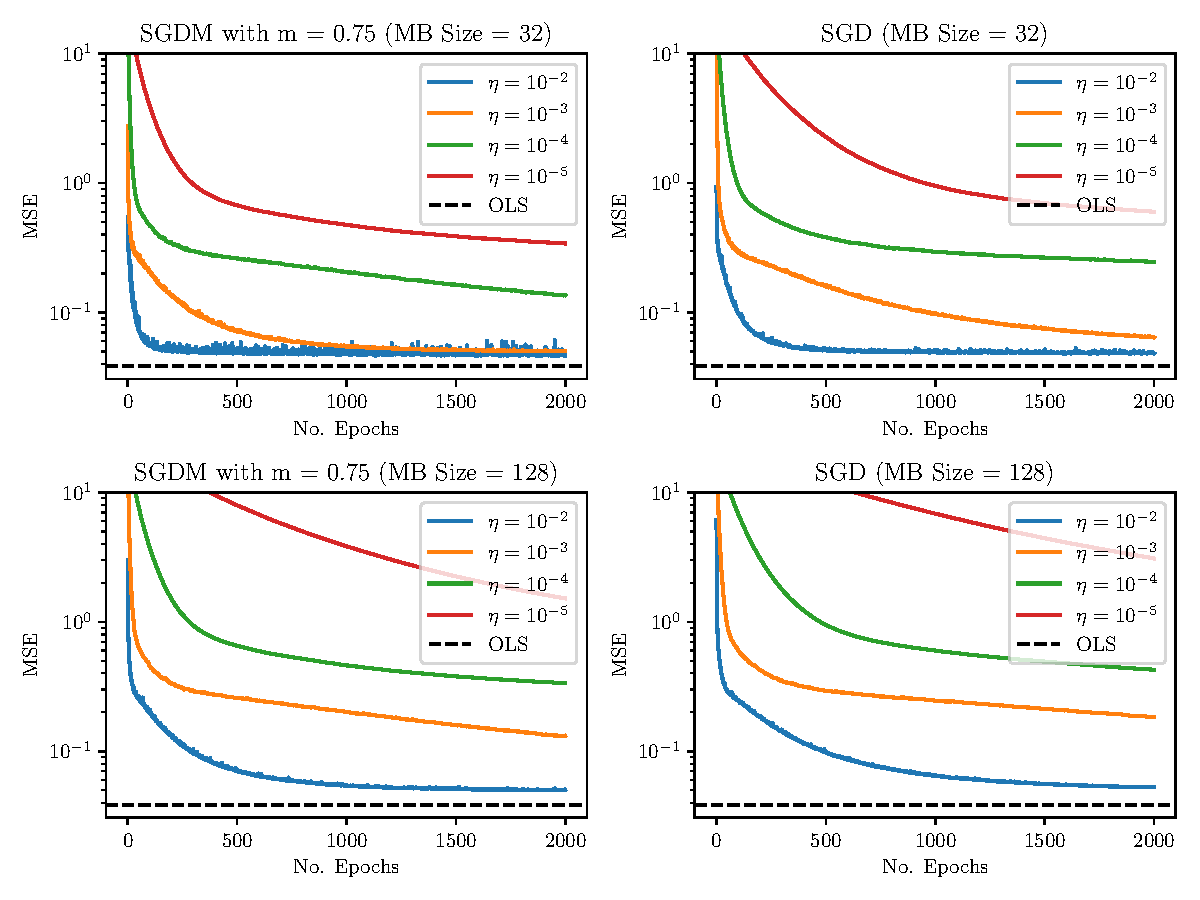
\includegraphics[width=\columnwidth]{SGD_learning_rate.pdf}
    \caption{\label{fig: SGD learning rate}Franke Function modeled as a 6th degree polynomial using an OLS type cost function optimized using Stochastic Gradient Descent with momentum for varying learning rates benchmarked against the analytic solution}
\end{figure}
Firstly, we look at all 4 plots in isolation, ignoring any comparison. We very clearly the effect of adjusting the learning rates $\eta$, leading to a quicker convergence. But notably; for $\eta = 10^{-2}$ in the case of $p=0.75$ and MB size $=32$, we see that once converged; the MSE becomes somewhat unstable, likely fluctuating around a minima. Here, the intuition is that whilst the SGD has been able to locate a local minima, it is unable to dive deeper into the minima due to its fixed learning rate, which if we draw the comparison of a ball rolling up and down in a quadratic well with a frictionless surface, it will never be able to settle further down the well for a given, constant energy. Where in this case, the learning rate is analogous to the energy of the ball. Therefore; once converged in such a way, lowering the learning rate is a necessity in order to converge to a lower MSE.

We then compare the vertically neighboring figures in Fig.~\ref{fig: SGD learning rate} by which may observe directly the result of varying the mini-batch size from $32$ to $128$, where the latter yields a more rapid initial convergence, but also a slightly more unstable exploration of the parameter space once converged, as exemplified by the SGDM plots on the left. More or less the same effect that we observe from varying increasing the learning rates, somewhat increasing our faith in the intuition proposed by \textcite{ManyBodyML}.

We compare the horizontally neighboring figures in Fig.~\ref{fig: SGD learning rate}, where we observe the effect of adding momentum. We see observe that the general effect of adding momentum is an increase in the convergence rate. In particular, for $\eta = 10^{-3}$ in the cases with $MB = 32$, we see the clear benefit; by yielding a quick and relatively stable convergence compared to the same learning rate without momentum.

We then turn our attention to Fig.~\ref{fig: SGD penalty}, where we observe the effect of adding a penalty parameter $\lambda$ to the cost function which punishes the weights, $\pmb w$ for having a large $L^2$ norm akin to Ridge regression \cite{4155_project_1}.
\begin{figure}
    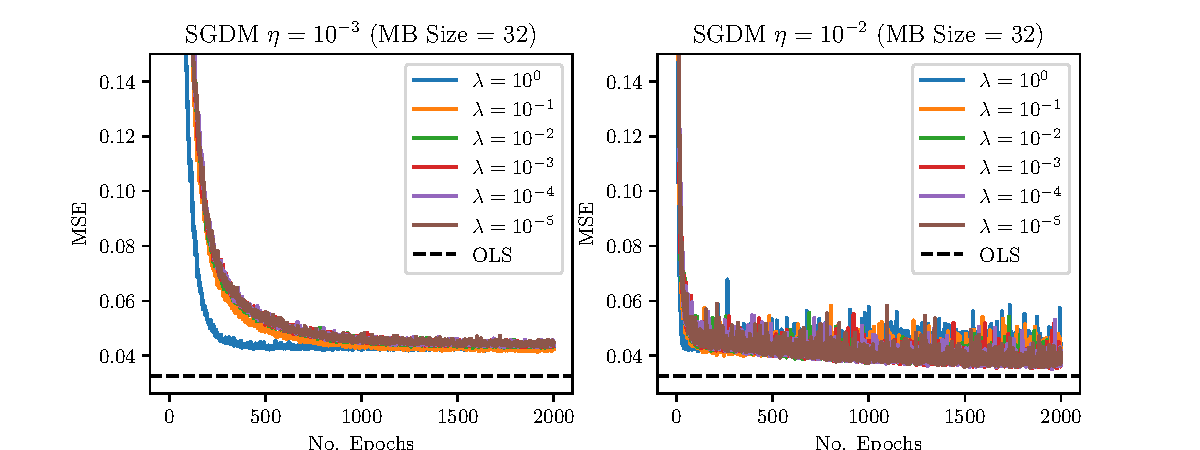
\includegraphics[width=\columnwidth]{SGD_learning_penalty.pdf}
    \caption{\label{fig: SGD penalty}Franke Function modeled as a 6th degree polynomial using an OLS type cost function optimized using Stochastic Gradient Descent with momentum $p=0.75$ for varying $L^2$ penalties $\lambda$ benchmarked against the analytic solution}
\end{figure}


\subsection{Classification of the MNIST dataset}
\noindent
We now turn to our analysis of the MNIST dataset \cite{lecun2010mnist}, consisting of $70\,000$ images each $28\times28$ pixels of labeled handwritten numbers, a small subset of which is shown in Fig.~\ref{fig: MNIST example}.
\begin{figure}[h!tb]
    \center
    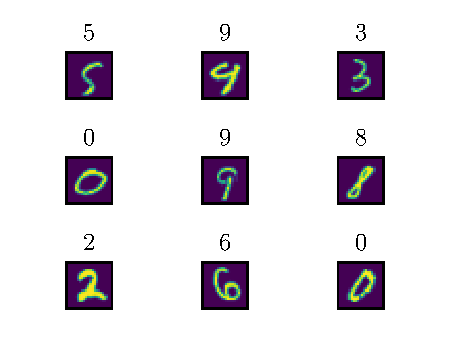
\includegraphics[width=.75\columnwidth]{MNIST_example.pdf}
    \caption{\label{fig: MNIST example}Examples from the MNIST data set}
\end{figure}
We wish to develop a model which can classify and assign a label to a previously unseen image as one of the 10 possible classes
\begin{equation*}
    \{0, 1, 2, 3, 4, 5, 6, 7, 8, 9\}
\end{equation*}
by the use of a FFNN and logistic regression, then to compare the performance of these two approaches. We randomly split the complete dataset into sets of training and testing data at a ratio of 80:20 respectively. Further, the labels are converted to one-hot form.

\subsubsection{FFNN Classification}
\noindent
We started by building a FFNN based classification model using the ReLU and Sigmoid activation functions for a single-layer neural network with varying number of neurons and the SoftMax activation function on the output layer, with its corresponding cost function Eqn.~\ref{eq:softmax_loss} as discussed in Sect.~\ref{sect: application of Neural Networks}. We then trained the network for 100 epochs with $\eta = 0.01$ and no penalty or momentum, monitoring the MSE wrt. testing set for each epoch. The result is seen in Fig.~\ref{fig: single layer MNIST relu and sigmoid}.

\begin{figure}[h!tb]
    \subfloat[ReLU]{
    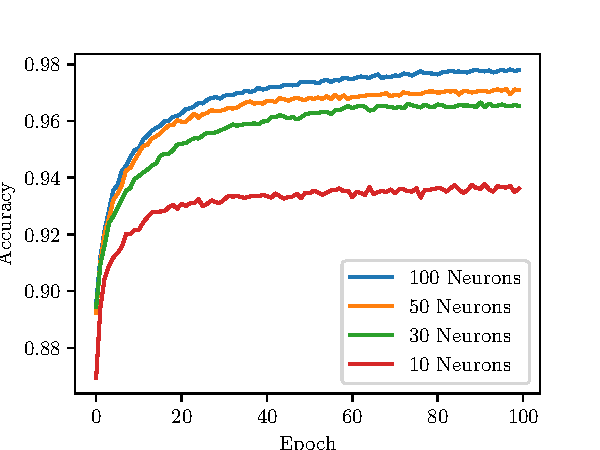
\includegraphics[width=.5\columnwidth]{MNIST_layers_ReLU.pdf}
    }
    \subfloat[Sigmoid]{
    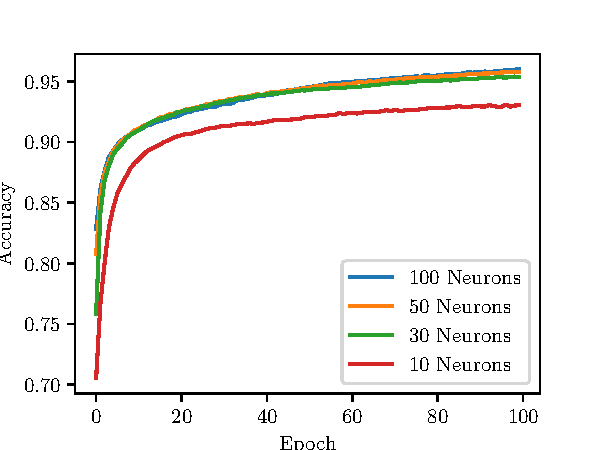
\includegraphics[width=.5\columnwidth]{MNIST_layers_Xavier.pdf}
    }
    \caption{\label{fig: single layer MNIST relu and sigmoid}FFNN trained on the MNIST dataset for a single-layer NN of various sizes for using both the ReLU (a) and Sigmoid (b) activation functions in the hidden layer and SoftMax in the outer layer. Notably, the final score for ReLU with 100 neurons was $\approx 0.978$}
\end{figure}
The first thing we observe is the relatively large jump in accuracy score when going from 10 neurons to 30, then much less so in the subsequent steps. We postulate then that 10 neurons in a single layer structure simply isn't able to recreate the full feature set of the data set, but the network gains freedom to do so, there is diminishing returns from adding further neurons.

%%%%% Logreg results and analysis
\subsubsection{Classification with Logistic Regression}

For our logistic-regression implementation we do a very similar analysis of the MNIST data. We once again use a 80/20 train/test-split and investigate the effect of various hyper-parameters on the obtained accuracy score for 100 epochs. Fig. \ref{fig:logreg_learning_rate} shows the score of the test set for the indicated choices of hyper-parameters, with the notable absence of any regularization penalty. The only noteworthy change in setup from the neural network is how we initialize the regression parameters $\mathbf{\beta}$. In the interest of simplicity we simply initialize them according to a standard normal distribution.We once again see that, for the better combinations of parameters, the performance fairly rapidly reaches fairly good scores, around 0.90 in these cases, before plateauing. Even the best combinatios have not yet fully converged, but the convergence rate rapidly slows down significantly; indicating that many, many more iterations are required to match the performance of our neural network, if it can be matched at all. Though not shown here (but see the logreg notebook in the test folder at \cite{4155_repo}), we have compared our results with the default logistic-regression classifier in sci-kit, and found nearly identical performance. Furthermore, the small discrepancy we did find vanishes completely when we downscale our $\mathbf{\beta}$-initialization, yielding a score of $\approx$ 0.92 as the best case after 100 epochs. It is eminently imaginable that further tuning could improve on this, but as it stands this is significantly worse than what we achieve with our neural network.


\begin{figure}
    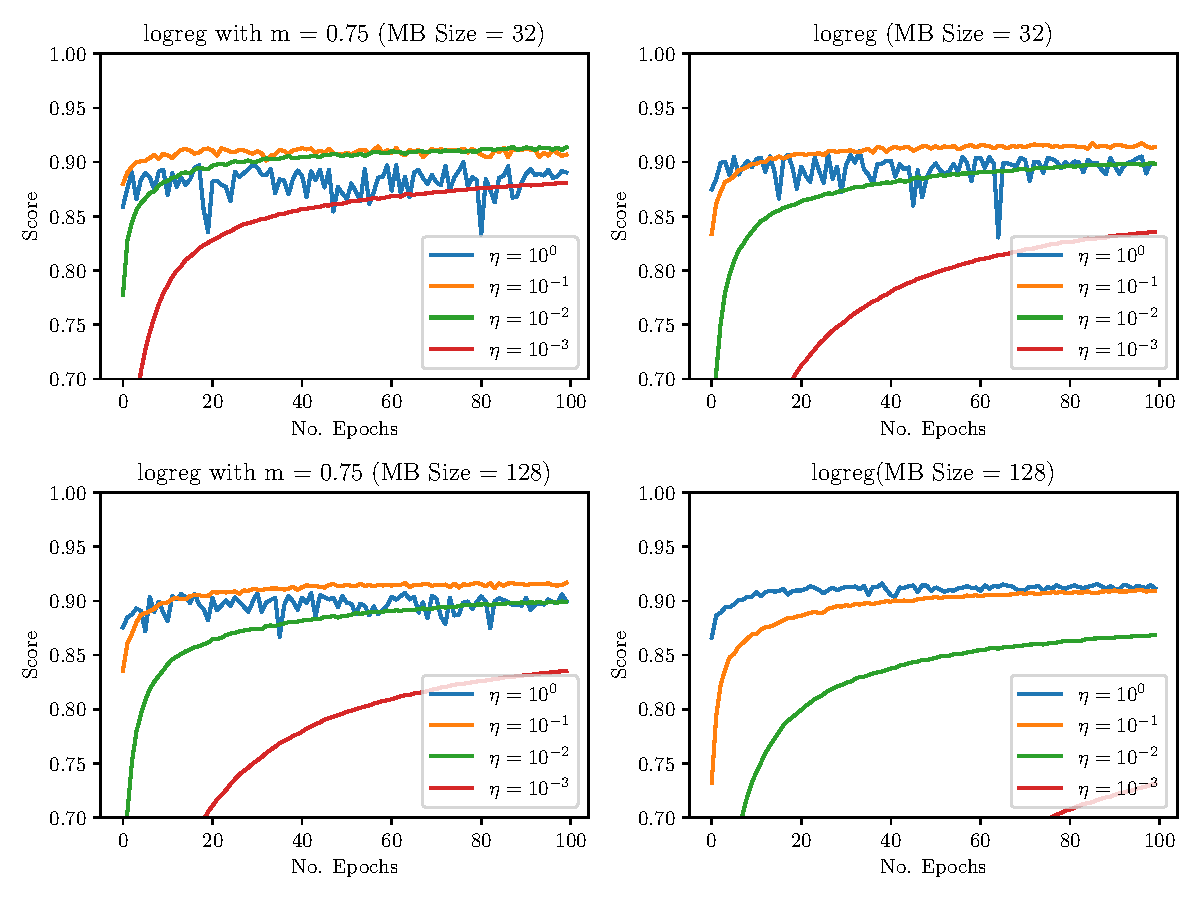
\includegraphics[width=\columnwidth]{logreg_learning_rate.pdf}
    \caption{\label{fig:logreg_learning_rate}Accuracy score on the test set for our logistic-regression method applied to the MNIST data set as a function of epochs run, for the indicated hyper-parameters and no regularization penalty.}
\end{figure}


We also take a look at the effects of adding a regularization parameter to our better choices of learning rates and minibatch-sizes. Fig. \ref{fig:logreg_regularization} shows the accuracy score on the test set for 100 epochs, using the indicated hyper-parameters such as the regularization parameters $\lambda$ and learning rates $\eta$, notably not adding a momentum hyper-parameter. We see that the regularization penalty does a remarkable job of killing the learning, keeping the results very stable around the result of the first epoch. Not shown here (but available for verification in the logreg notebook at \cite{4155_repo}), we find that the addition of a momentum term of 0.75 does make our best combinations immediately (i.e. already after just one epoch) start, and stay stable, at an accuracy score of $\approx$ 0.90-0.92, consistent with the default performance of sci-kit's logistic-regression classifier. 

In summary, we find that logistic-regression classifiers are capable of very quickly getting quite reasonable (accuracy score on test set of $\approx$ 0.91) performance, but that further refinement is slow as molasses without further fine-tuning. Meanwhile our neural network can fairly easily achieve a significantly better performance in the same number of epochs. The only advantage of the logistic-regression classifier seems to be that it can pretty much start (after one epoch of training) at close to its best performance when using regularization and momentum, while the neural network does require som epochs of training before it really gives superior performance.


\begin{figure}
    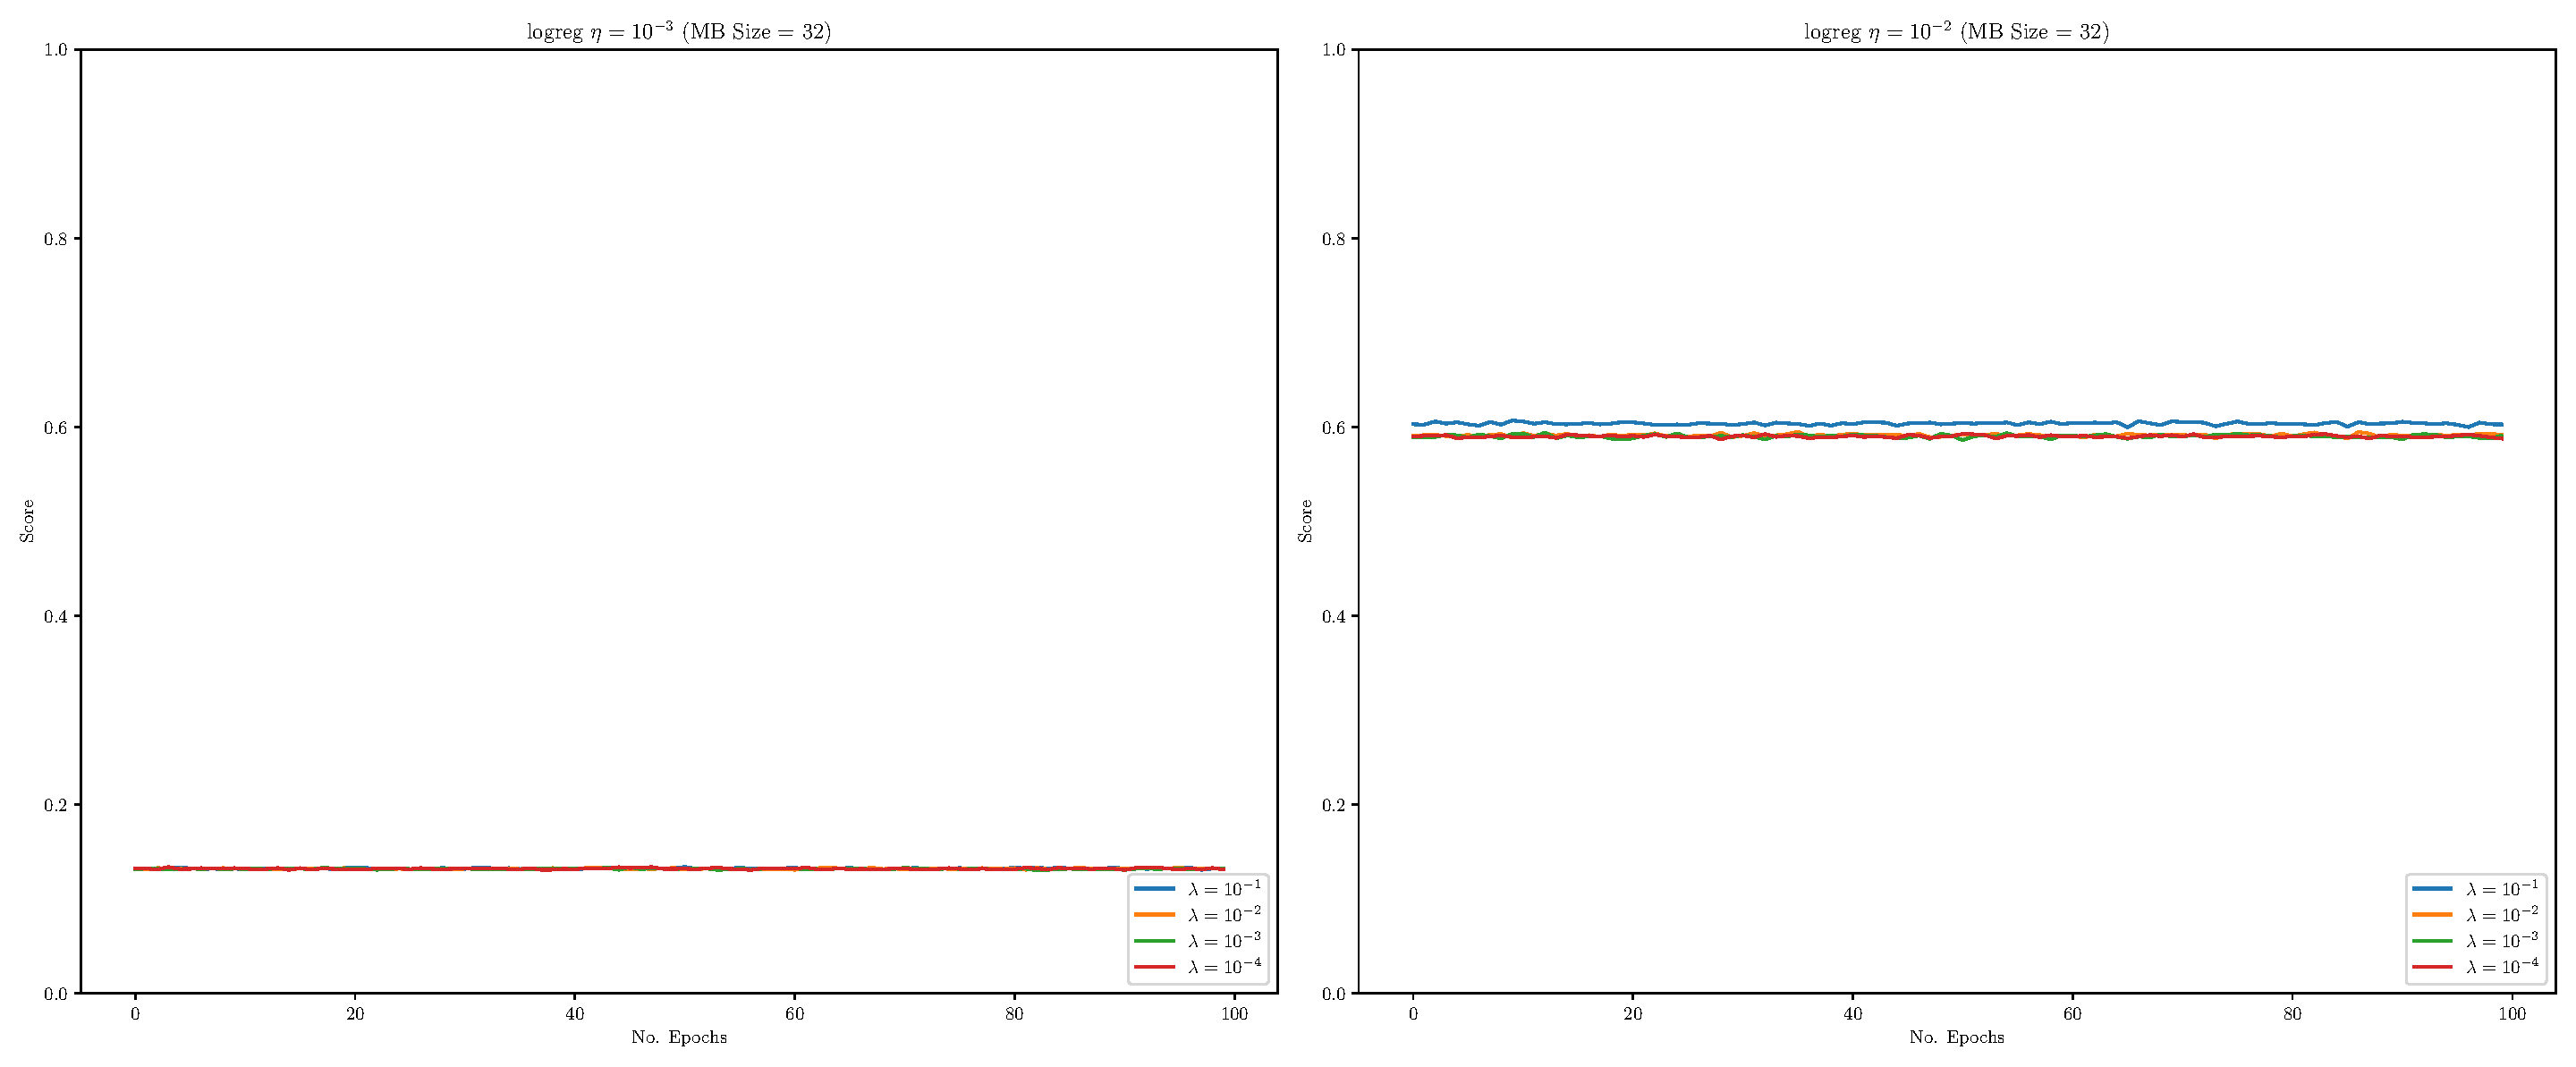
\includegraphics[width=\columnwidth]{logreg_regularization.pdf}
    \caption{\label{fig:logreg_regularization}Accuracy score on the test set for our logistic-regression method applied to the MNIST data set as a function of epochs runs for the indicated hyper-parameters and no momentum.}
\end{figure}

%%%%%%%% End logreg results and analysis


\section{Conclusion}

%%%%%%% Conclusion

With the massive flexibility and freedom granted by the direct dearth of hyper-parameters to consider, it is very difficult to make definite statements about which method is the optimal onefor each problem. There may very well be far superior combinations of hyper-parameters, both in terms of speed and accuracy, than those we have tested for all the methods we have investigated in this paper. We can, however, highlight some considerations and tendencies based on our experiences throughout this work.

% Regression type: main findings: learning rate, activation functions, regularization, convergence time and predictive performance

% Classification type: main findings: learning rate, activation functions, regularization, convergence time and predictive performance

In summary, if you are pressed for time and want something that very easily just works, and works pretty well, your best bet seems to be linear-regression methods for predicting terrain-type data. There is improvement to be had from neural networks, but the cost in time spent tuning is steep. For the classification case both the neural network and logistic regression are fairly easy to get going well, but the neural network does have a marked performance with minimal mucking around required.

%%%%%%%%%

\onecolumngrid
\bibliography{bibfile}
\newpage
\twocolumngrid
\appendix
\end{document}
